\section{Study 1: calibration-marginal versus plug-in adaptive testing}
\label{sec:study1}
\label{sec:results}

\subsection{Decisions under the frozen plan, and with dependent targets}
Table~\ref{tab:confirm} reports the four frozen contrasts at $N=8$ and
Table~\ref{tab:allN} all panel sizes. \ResultsHypotheses

\begin{table}[tbp]
\centering\footnotesize
\caption{Study 1 at the primary panel size $N=8$: relative improvement (\%) of EOST-M over the baseline of each hypothesis (log loss for H1--H2, score error for H3, $|\mathrm{coverage}-0.9|$ for H4); * Holm-significant in favour of EOST-M (none in favour of a baseline). Last row: benchmarks significant for EOST-M / for the baseline, and the frozen decision. Full statistics in Table~\ref{tab:confirmfull}.}
\label{tab:confirm}
\setlength{\tabcolsep}{5pt}
\begin{tabular}{@{}lrcccc@{}}
\toprule
 & & H1 & H2 & H3 & H4 \\
Benchmark & targets & vs Entropy:mg & vs MFI:pi & vs Naive & vs MFI:pi \\
\midrule
GSM8K & 60 & $+2.7$* & $+2.4$ & $+16.8$ & $+11.6$ \\
ARC-C & 60 & $+0.4$ & $+4.7$* & $+61.0$* & $+41.6$* \\
HellaSwag & 60 & $+5.5$* & $+9.6$* & $+68.4$* & $+46.8$* \\
WinoGrande & 60 & $+3.1$* & $+4.9$* & $+53.4$* & $+57.3$* \\
MMLU & 60 & $+2.9$* & $+5.0$* & $+55.3$* & $+59.0$* \\
SWE-bench V. & 60 & $+0.7$ & $+6.1$* & $+46.9$* & $+31.7$* \\
LiveCodeBench & 28 & $+1.0$ & $+6.4$* & $+51.3$* & $+48.1$* \\
CRUXEval-O & 31 & $+0.5$ & $+5.4$* & $+57.7$* & $+33.4$* \\
\midrule
decision & & 4/0 not supported & 7/0 supported & 7/0 supported & 7/0 supported \\
\bottomrule
\end{tabular}
\end{table}

\begin{table}[tbp]
\centering\footnotesize
\caption{Confirmatory tests at every panel size: benchmarks with a Holm-significant difference favouring EOST-M / favouring the baseline / tested, and (in parentheses) the median relative improvement across benchmarks.}
\label{tab:allN}
\begin{tabular}{@{}lccccc@{}}
\toprule
 & $N=4$ & $N=8$ & $N=16$ & $N=32$ & $N=64$ \\
\midrule
H1 & 7/0/8 ($+2.5$\%) & 4/0/8 ($+1.9$\%) & 7/0/8 ($+1.5$\%) & 5/0/6 ($+2.1$\%) & 5/0/6 ($+1.8$\%) \\
H2 & 8/0/8 ($+7.1$\%) & 7/0/8 ($+5.2$\%) & 3/0/8 ($+3.6$\%) & 1/0/6 ($+1.9$\%) & 0/0/6 ($+1.1$\%) \\
H3 & 7/0/8 ($+45.9$\%) & 7/0/8 ($+54.4$\%) & 8/0/8 ($+60.9$\%) & 6/0/6 ($+62.5$\%) & 6/0/6 ($+62.1$\%) \\
H4 & 7/0/8 ($+56.4$\%) & 7/0/8 ($+44.2$\%) & 4/0/8 ($+29.4$\%) & 3/0/6 ($+21.5$\%) & 1/0/6 ($+10.3$\%) \\
\bottomrule
\end{tabular}
\end{table}


Targets of one family are not independent, and on the Open LLM Leaderboard they are
numerous: hundreds of systems are fine-tunes or merges of a few base models.
Table~\ref{tab:clusters} repeats every contrast with families as units. With heuristic
families the frozen decisions are unchanged. With strict clusters---which also merge
near-duplicates found from the verdicts and leave between \CluStrictUnitsMin\ and
\CluStrictUnitsMax\ units per benchmark---H3 and H4 remain supported, but H2 is
significant on \CluHTwoStrFav\ of 8 benchmarks only, below the frozen threshold of five,
although its median effect is unchanged (\CluHTwoStrMed\%, 95\% cluster-bootstrap interval
\CluHTwoCILo--\CluHTwoCIHi\%). The effect of marginalization on prediction is therefore
not in doubt, but the per-benchmark significance claimed with targets as units overstates
the evidence; study~2 was designed with one target per cluster to settle the question.

\IfFileExists{tables/clusters.tex}{\begin{table}[tbp]
\centering\footnotesize
\caption{Study 1 with dependent targets taken into account (post hoc). Benchmarks with a Holm-significant difference favouring EOST-M / favouring the baseline at $N=8$, with the frozen decision in parentheses, when the unit of analysis is the target (frozen plan), the heuristic family or the strict cluster (targets averaged within unit; same 144-test Holm family). Last column: median relative improvement over benchmarks with strict clusters as units, and its 95\% cluster-bootstrap interval.}
\label{tab:clusters}
\setlength{\tabcolsep}{3.5pt}
\begin{tabular}{@{}llcccc@{}}
\toprule
 & Contrast & target & heuristic family & strict cluster & median \% [95\% CI] \\
\midrule
H1 & EIG:mg vs Entropy:mg (log loss) & 4/0 (no) & 4/0 (no) & 4/0 (no) & 1.8 [1.3, 2.5] \\
H2 & EIG:mg vs MFI:pi (log loss) & 7/0 (yes) & 5/0 (yes) & 4/0 (no) & 5.4 [4.3, 6.4] \\
H3 & EIG:mg vs Naive (score IAE) & 7/0 (yes) & 7/0 (yes) & 7/0 (yes) & 55.4 [50.8, 57.6] \\
H4 & EIG:mg vs MFI:pi ($|\mathrm{cov}-0.9|$) & 7/0 (yes) & 5/0 (yes) & 5/0 (yes) & 44.6 [37.0, 50.5] \\
\bottomrule
\end{tabular}
\end{table}
}{}
\begin{table}[tbp]
\centering\footnotesize
\caption{Study 1 in full at the primary panel size $N=8$. Per-target means over 5 replicates; $n$ targets; improvement is relative to the baseline (positive favours EOST-M); W/L wins/losses over targets; $r_{rb}$ matched-pairs rank-biserial; $p$ two-sided Wilcoxon, Holm-adjusted over the whole family; $\uparrow$/$\downarrow$ significant in favour of EOST-M/baseline.}
\label{tab:confirmfull}
\setlength{\tabcolsep}{4pt}
\begin{tabular}{@{}lrrrrrrl@{}}
\toprule
Benchmark & $n$ & Baseline & EOST-M & Improv. & W/L & $r_{rb}$ & $p_{\rm Holm}$ \\
\midrule
\multicolumn{8}{@{}l}{\textit{H1: EIG:mg vs Entropy:mg (log loss)}}\\
\quad GSM8K & 60 & 0.3885 & 0.3779 & $+2.7$\% & 52/8 & $+0.88$ & $<10^{-4}$ $\uparrow$\\
\quad ARC-C & 60 & 0.3478 & 0.3464 & $+0.4$\% & 39/21 & $+0.37$ & 0.369 \\
\quad HellaSwag & 60 & 0.1880 & 0.1777 & $+5.5$\% & 55/5 & $+0.90$ & $<10^{-4}$ $\uparrow$\\
\quad WinoGrande & 60 & 0.3792 & 0.3674 & $+3.1$\% & 52/8 & $+0.78$ & $<10^{-4}$ $\uparrow$\\
\quad MMLU & 60 & 0.4817 & 0.4677 & $+2.9$\% & 53/7 & $+0.89$ & $<10^{-4}$ $\uparrow$\\
\quad SWE-bench V. & 60 & 0.3838 & 0.3811 & $+0.7$\% & 41/19 & $+0.35$ & 0.560 \\
\quad LiveCodeBench & 28 & 0.2813 & 0.2784 & $+1.0$\% & 16/12 & $+0.32$ & 1.000 \\
\quad CRUXEval-O & 31 & 0.3838 & 0.3817 & $+0.5$\% & 22/9 & $+0.31$ & 1.000 \\
\multicolumn{8}{@{}r}{\footnotesize decision rule: 4/8 favour EOST-M, 0 favour baseline $\Rightarrow$ \textbf{not supported}}\\[2pt]
\multicolumn{8}{@{}l}{\textit{H2: EIG:mg vs MFI:pi (log loss)}}\\
\quad GSM8K & 60 & 0.3874 & 0.3779 & $+2.4$\% & 33/27 & $+0.28$ & 1.000 \\
\quad ARC-C & 60 & 0.3634 & 0.3464 & $+4.7$\% & 45/15 & $+0.70$ & 0.0002 $\uparrow$\\
\quad HellaSwag & 60 & 0.1967 & 0.1777 & $+9.6$\% & 41/19 & $+0.64$ & 0.0010 $\uparrow$\\
\quad WinoGrande & 60 & 0.3865 & 0.3674 & $+4.9$\% & 38/22 & $+0.52$ & 0.020 $\uparrow$\\
\quad MMLU & 60 & 0.4922 & 0.4677 & $+5.0$\% & 44/16 & $+0.63$ & 0.0012 $\uparrow$\\
\quad SWE-bench V. & 60 & 0.4060 & 0.3811 & $+6.1$\% & 48/12 & $+0.78$ & $<10^{-4}$ $\uparrow$\\
\quad LiveCodeBench & 28 & 0.2973 & 0.2784 & $+6.4$\% & 19/9 & $+0.70$ & 0.032 $\uparrow$\\
\quad CRUXEval-O & 31 & 0.4036 & 0.3817 & $+5.4$\% & 26/5 & $+0.81$ & 0.0010 $\uparrow$\\
\multicolumn{8}{@{}r}{\footnotesize decision rule: 7/8 favour EOST-M, 0 favour baseline $\Rightarrow$ \textbf{supported}}\\[2pt]
\multicolumn{8}{@{}l}{\textit{H3: EIG:mg vs Naive (score IAE)}}\\
\quad GSM8K & 60 & 0.0526 & 0.0438 & $+16.8$\% & 41/19 & $+0.46$ & 0.084 \\
\quad ARC-C & 60 & 0.0732 & 0.0285 & $+61.0$\% & 60/0 & $+1.00$ & $<10^{-4}$ $\uparrow$\\
\quad HellaSwag & 60 & 0.0572 & 0.0181 & $+68.4$\% & 58/2 & $+0.99$ & $<10^{-4}$ $\uparrow$\\
\quad WinoGrande & 60 & 0.0630 & 0.0293 & $+53.4$\% & 58/2 & $+1.00$ & $<10^{-4}$ $\uparrow$\\
\quad MMLU & 60 & 0.0727 & 0.0325 & $+55.3$\% & 58/2 & $+0.99$ & $<10^{-4}$ $\uparrow$\\
\quad SWE-bench V. & 60 & 0.0666 & 0.0353 & $+46.9$\% & 55/5 & $+0.94$ & $<10^{-4}$ $\uparrow$\\
\quad LiveCodeBench & 28 & 0.0591 & 0.0288 & $+51.3$\% & 28/0 & $+1.00$ & $<10^{-4}$ $\uparrow$\\
\quad CRUXEval-O & 31 & 0.0734 & 0.0311 & $+57.7$\% & 31/0 & $+1.00$ & $<10^{-4}$ $\uparrow$\\
\multicolumn{8}{@{}r}{\footnotesize decision rule: 7/8 favour EOST-M, 0 favour baseline $\Rightarrow$ \textbf{supported}}\\[2pt]
\multicolumn{8}{@{}l}{\textit{H4: EIG:mg vs MFI:pi ($|\mathrm{cov}-0.9|$)}}\\
\quad GSM8K & 60 & 0.2451 & 0.2166 & $+11.6$\% & 38/20 & $+0.22$ & 1.000 \\
\quad ARC-C & 60 & 0.2935 & 0.1715 & $+41.6$\% & 49/10 & $+0.85$ & $<10^{-4}$ $\uparrow$\\
\quad HellaSwag & 60 & 0.3178 & 0.1690 & $+46.8$\% & 48/12 & $+0.76$ & $<10^{-4}$ $\uparrow$\\
\quad WinoGrande & 60 & 0.3990 & 0.1704 & $+57.3$\% & 54/6 & $+0.96$ & $<10^{-4}$ $\uparrow$\\
\quad MMLU & 60 & 0.3880 & 0.1593 & $+59.0$\% & 55/5 & $+0.92$ & $<10^{-4}$ $\uparrow$\\
\quad SWE-bench V. & 60 & 0.2502 & 0.1710 & $+31.7$\% & 41/19 & $+0.52$ & 0.020 $\uparrow$\\
\quad LiveCodeBench & 28 & 0.3091 & 0.1604 & $+48.1$\% & 21/7 & $+0.77$ & 0.0072 $\uparrow$\\
\quad CRUXEval-O & 31 & 0.2680 & 0.1786 & $+33.4$\% & 22/9 & $+0.67$ & 0.048 $\uparrow$\\
\multicolumn{8}{@{}r}{\footnotesize decision rule: 7/8 favour EOST-M, 0 favour baseline $\Rightarrow$ \textbf{supported}}\\[2pt]
\bottomrule
\end{tabular}
\end{table}


\subsection{Where the gain comes from}
\ResultsFactorial\ The gain of EOST-M over plug-in Fisher CAT also decreases
monotonically with the panel size on every benchmark---largest with four calibrators,
nearly gone with 64 (Figure~\ref{fig:heatmap})---as Proposition~\ref{prop:cap}
predicts, since the uncertainty of item difficulties shrinks as calibrators are added.
\ResultsDiagnostics

\begin{table}[tbp]
\centering\footnotesize
\caption{Decomposing the gain over plug-in Fisher CAT (MFI:pi): selection criterion (entropy vs.\ EIG) $\times$ measurement model (plug-in vs.\ calibration-marginal). Median across confirmatory benchmarks of the relative improvement over MFI:pi, in \%; $B$ = number of benchmarks.}
\label{tab:factorial}
\setlength{\tabcolsep}{3.5pt}
\begin{tabular}{@{}rrrrrrrrrr@{}}
\toprule
 & & \multicolumn{4}{c}{holdout log loss} & \multicolumn{4}{c}{score IAE} \\
\cmidrule(lr){3-6}\cmidrule(lr){7-10}
$N$ & $B$ & Ent:pi & EIG:pi & Ent:mg & EIG:mg & Ent:pi & EIG:pi & Ent:mg & EIG:mg \\
\midrule
4 & 8 & $-0.8$ & $-0.1$ & $+5.0$ & $+7.1$ & $-12.3$ & $-0.8$ & $-15.2$ & $+11.7$ \\
8 & 8 & $-1.8$ & $0.0$ & $+4.4$ & $+5.2$ & $-17.5$ & $+0.7$ & $-9.2$ & $+7.5$ \\
16 & 8 & $-1.4$ & $0.0$ & $+2.0$ & $+3.6$ & $-18.7$ & $-0.7$ & $-10.9$ & $+5.9$ \\
32 & 6 & $-1.8$ & $0.0$ & $-0.5$ & $+1.9$ & $-23.4$ & $+0.2$ & $-22.8$ & $+7.4$ \\
64 & 6 & $-2.0$ & $+0.1$ & $-1.3$ & $+1.1$ & $-17.5$ & $+0.6$ & $-16.7$ & $+6.6$ \\
\bottomrule
\end{tabular}
\end{table}


\begin{figure}[tbp]
\centering
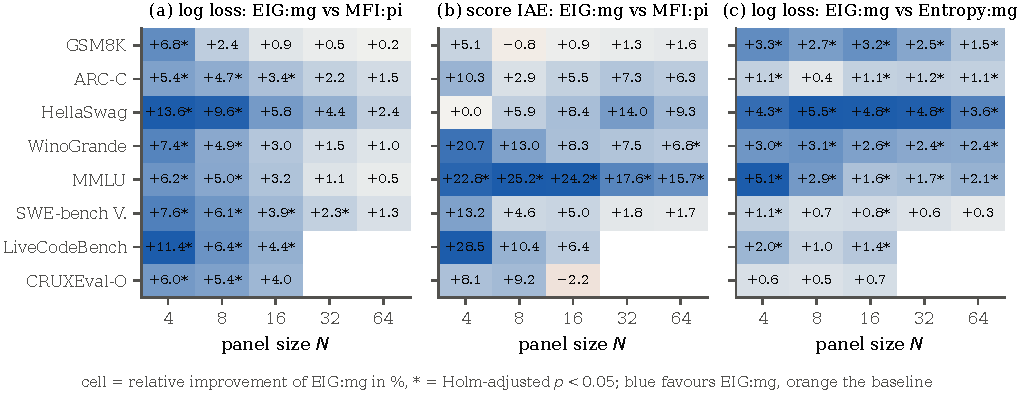
\includegraphics[width=\linewidth]{figures/heatmap_improvement.pdf}
\caption{Relative improvement (\%) of EIG:mg over the baseline for every benchmark and calibration-panel size; * marks Holm-adjusted $p<0.05$ (panels a and c: confirmatory family; panel b: secondary family). Blue favours EIG:mg.}
\label{fig:heatmap}
\end{figure}

\begin{figure}[tbp]
\centering
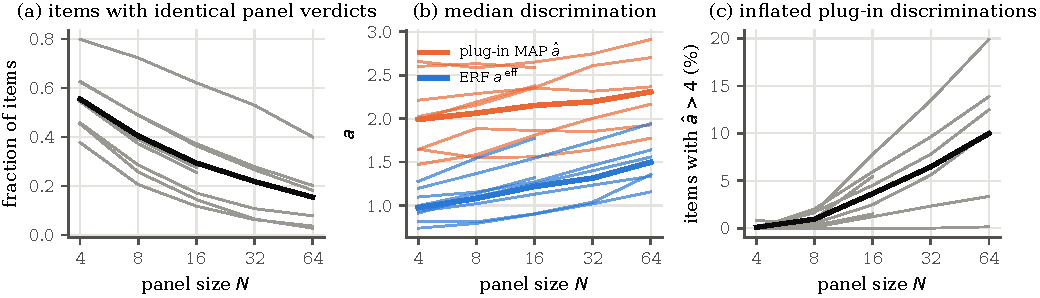
\includegraphics[width=\linewidth]{figures/calibration_diagnostics.pdf}
\caption{Calibration diagnostics on the study-1 benchmarks (thin lines: individual benchmarks; thick: mean). (a) Fraction of items that every calibrator answered identically, whose difficulty is identified only through the prior. (b) Median plug-in discrimination versus the effective discrimination of the expected response function. (c) Fraction of items whose plug-in discrimination exceeds 4 under the empirical-Bayes prior.}
\label{fig:diag}
\end{figure}

\begin{figure}[tbp]
\centering
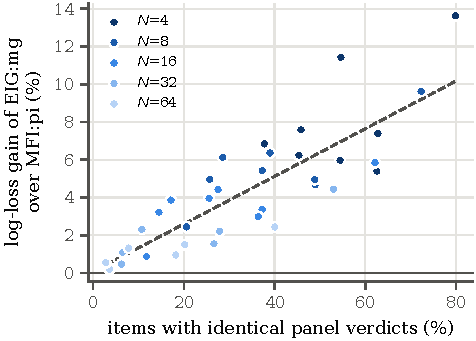
\includegraphics[width=0.55\linewidth]{figures/mechanism.pdf}
\caption{Exploratory: the log-loss gain of EIG:mg over plug-in Fisher CAT grows with the fraction of items that the calibration panel cannot locate (identical verdicts across calibrators). One point per benchmark and panel size; dashed: least-squares line.}
\label{fig:mechanism}
\end{figure}

\subsection{Learning curves}\label{sec:curves}
\ResultsCurves\ \ResultsEfficiency\ Table~\ref{tab:full} gives the held-out log loss, the
score error and the coverage of six of the policies on every bank, real or synthetic, and
every panel size, and Figure~\ref{fig:curves-brier} the holdout Brier score as items are
administered.

\begin{figure}[tbp]
\centering
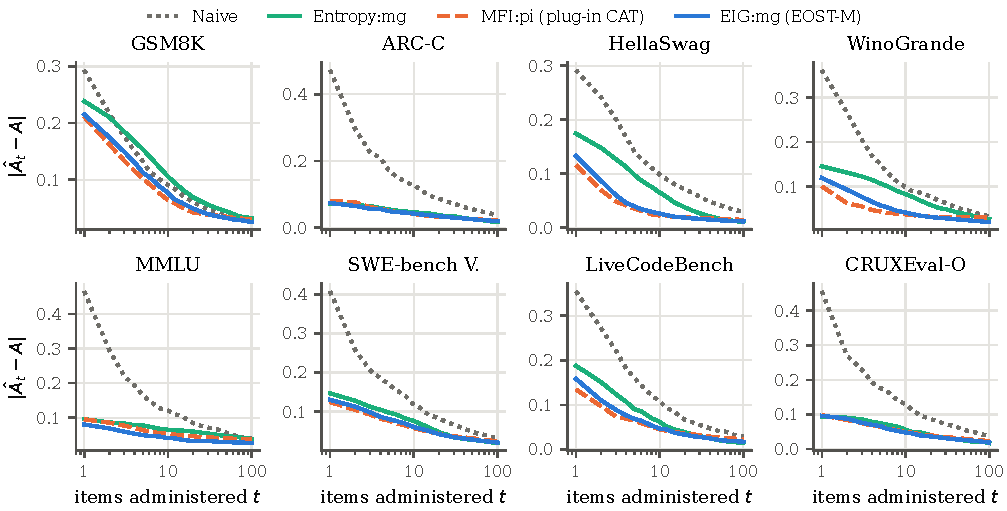
\includegraphics[width=\linewidth]{figures/curves_err_N8.pdf}
\caption{Absolute error of the full-bank score estimate as items are administered ($N=8$; mean over targets of per-target means over 5 replicates; logarithmic $t$ axis).}
\label{fig:curves-err}
\end{figure}

\begin{figure}[tbp]
\centering
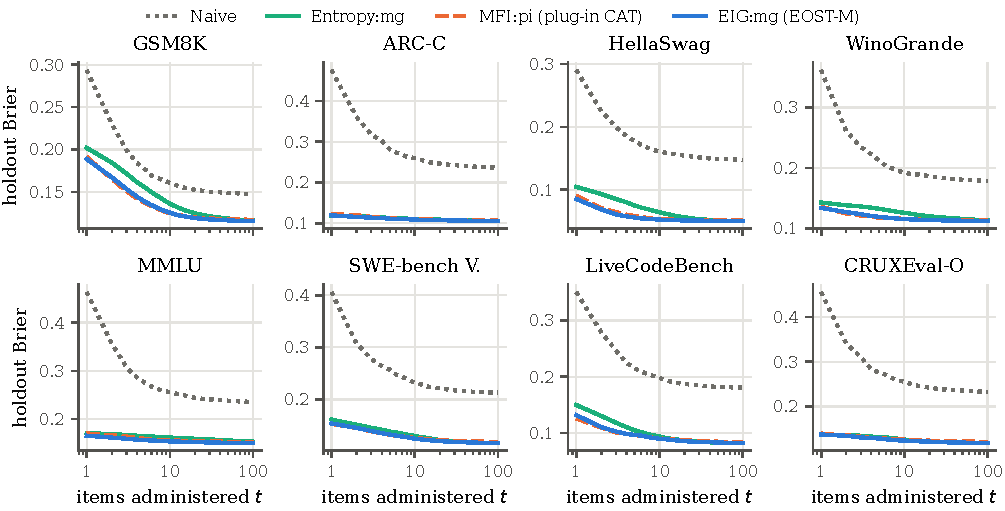
\includegraphics[width=\linewidth]{figures/curves_brier_N8.pdf}
\caption{Holdout Brier score as items are administered ($N=8$).}
\label{fig:curves-brier}
\end{figure}

\begin{table}[tbp]
\centering\footnotesize
\caption{All twelve policies at $N=8$, averaged over the eight confirmatory benchmarks (mean of per-benchmark means; in parentheses the mean rank across benchmarks, 1 = best). IAE: integrated absolute error of the full-bank score; $|\mathrm{cov}-0.9|$: miscalibration of the 90\% interval; $t_{0.03}$: sustained items-to-tolerance at $\varepsilon=0.03$ (101 = never).}
\label{tab:policies}
\setlength{\tabcolsep}{4pt}
\begin{tabular}{@{}lllll@{}}
\toprule
Policy & holdout log loss & score IAE & $|\mathrm{cov}-0.9|$ & $t_{0.03}$ \\
\midrule
Naive & -- & 0.0647 (11.5) & 0.0644 (1.1) & 86.3 (11.6) \\
Random:pi & 0.3720 (10.4) & 0.0424 (9.8) & 0.0972 (2.8) & 71.2 (10.0) \\
Random:mg & 0.3564 (6.1) & 0.0432 (10.0) & 0.0897 (2.2) & 71.5 (10.4) \\
Entropy:pi & 0.3724 (10.0) & 0.0398 (8.9) & 0.1598 (6.6) & 61.5 (8.8) \\
Entropy:mg & 0.3543 (5.6) & 0.0394 (8.4) & 0.1190 (4.9) & 64.0 (8.9) \\
MFI:pi (plug-in CAT) & 0.3666 (8.1) & 0.0341 (6.2) & 0.3088 (10.8) & 53.4 (5.1) \\
MFI:mg & 0.3470 (2.5) & 0.0301 (2.5) & 0.1677 (6.6) & 50.3 (4.0) \\
PWFI:mg & 0.3469 (2.1) & 0.0301 (2.1) & 0.1686 (7.1) & 49.9 (3.1) \\
EIG:pi & 0.3665 (7.8) & 0.0339 (6.0) & 0.3142 (11.4) & 53.6 (4.8) \\
EIG:mg \textbf{(EOST-M)} & 0.3473 (3.0) & 0.0309 (3.8) & 0.1746 (7.6) & 50.5 (3.8) \\
EVR:pi & 0.3665 (8.0) & 0.0340 (6.0) & 0.3051 (10.5) & 53.0 (4.2) \\
EVR:mg & 0.3471 (2.4) & 0.0303 (2.9) & 0.1664 (6.4) & 50.0 (3.4) \\
\bottomrule
\end{tabular}
\end{table}

\begin{table}[tbp]
\centering\footnotesize
\caption{Items needed to match the full-bank score error of 100 uniformly sampled items (Naive): first checkpoint $t$ at which the mean $|\hat A_t-A|$ over targets falls below the Naive error at $t=100$, at the primary panel size $N=8$ and at the largest panel available for the benchmark.}
\label{tab:efficiency}
\begin{tabular}{@{}lrrrrrr@{}}
\toprule
Benchmark & $N$ & Naive error @100 & Entropy:mg & MFI:pi & EIG:mg & EVR:mg \\
\midrule
GSM8K & 8 & 0.0296 & $>$100 & $>$100 & 70 & 80 \\
 & 64 & 0.0258 & $>$100 & 90 & 80 & 80 \\
\addlinespace[2pt]
ARC-C & 8 & 0.0364 & 25 & 15 & 20 & 12 \\
 & 64 & 0.0408 & 12 & 5 & 3 & 3 \\
\addlinespace[2pt]
HellaSwag & 8 & 0.0295 & 30 & 8 & 8 & 10 \\
 & 64 & 0.0306 & 10 & 3 & 3 & 4 \\
\addlinespace[2pt]
WinoGrande & 8 & 0.0326 & 80 & 20 & 20 & 15 \\
 & 64 & 0.0311 & 30 & 8 & 6 & 5 \\
\addlinespace[2pt]
MMLU & 8 & 0.0395 & 100 & 60 & 15 & 12 \\
 & 64 & 0.0396 & 25 & 6 & 5 & 6 \\
\addlinespace[2pt]
SWE-bench V. & 8 & 0.0334 & 40 & 50 & 40 & 40 \\
 & 64 & 0.0314 & 30 & 40 & 40 & 30 \\
\addlinespace[2pt]
LiveCodeBench & 8 & 0.0305 & 30 & 40 & 25 & 30 \\
 & 16 & 0.0298 & 25 & 20 & 15 & 20 \\
\addlinespace[2pt]
CRUXEval-O & 8 & 0.0359 & 25 & 30 & 25 & 20 \\
 & 16 & 0.0379 & 25 & 10 & 10 & 10 \\
\addlinespace[2pt]
\bottomrule
\end{tabular}
\end{table}


\ResultsLate

\begin{figure}[tbp]
\centering
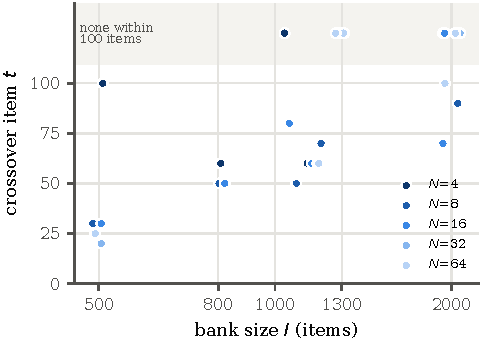
\includegraphics[width=0.55\linewidth]{figures/crossover.pdf}
\caption{Exploratory test of the regime change of Proposition~\ref{prop:evr}: the item after which entropy selection under the marginal model has a lower score error than EIG:mg at every later checkpoint, against the size of the bank. One point per benchmark and panel size (jittered horizontally); shaded band: no crossover within the 100-item budget.}
\label{fig:crossover}
\end{figure}

\begin{table}[p]
\centering\scriptsize
\caption{Full results: holdout log loss / score IAE / coverage of the 90\% interval (per-target means, then averaged over targets; leading zeros omitted).}
\label{tab:full}
\setlength{\tabcolsep}{2.5pt}
\begin{tabular}{@{}lrllllll@{}}
\toprule
Bank & $N$ & Naive & Entropy:mg & MFI:pi (plug-in CAT) & EIG:pi & EIG:mg & EVR:mg \\
\midrule
GSM8K & 4 & --/.051/.92 & .422/.069/.62 & .438/.054/.60 & .438/.055/.58 & .408/.052/.67 & .411/.055/.65 \\
GSM8K & 8 & --/.053/.89 & .388/.058/.67 & .387/.043/.67 & .387/.042/.68 & .378/.044/.70 & .379/.044/.69 \\
GSM8K & 16 & --/.054/.90 & .367/.053/.70 & .358/.038/.70 & .358/.038/.70 & .355/.037/.73 & .356/.039/.72 \\
GSM8K & 32 & --/.053/.91 & .348/.045/.73 & .341/.035/.70 & .341/.035/.70 & .340/.034/.73 & .341/.035/.73 \\
GSM8K & 64 & --/.053/.89 & .334/.041/.75 & .330/.035/.68 & .330/.035/.68 & .329/.035/.70 & .329/.035/.70 \\
\addlinespace[1pt]
ARC-C & 4 & --/.072/.90 & .383/.038/.87 & .400/.037/.56 & .401/.037/.58 & .378/.033/.78 & .377/.033/.77 \\
ARC-C & 8 & --/.073/.90 & .348/.029/.89 & .363/.029/.61 & .364/.030/.61 & .346/.029/.74 & .346/.027/.76 \\
ARC-C & 16 & --/.075/.89 & .325/.027/.87 & .332/.026/.58 & .332/.025/.59 & .321/.024/.70 & .321/.023/.71 \\
ARC-C & 32 & --/.076/.88 & .310/.026/.86 & .314/.024/.57 & .314/.024/.57 & .307/.022/.65 & .307/.023/.65 \\
ARC-C & 64 & --/.074/.88 & .303/.026/.82 & .304/.024/.55 & .303/.024/.55 & .299/.023/.60 & .299/.023/.60 \\
\addlinespace[1pt]
HellaSwag & 4 & --/.057/.90 & .213/.033/.76 & .236/.023/.60 & .237/.023/.58 & .204/.023/.78 & .205/.024/.80 \\
HellaSwag & 8 & --/.057/.90 & .188/.029/.80 & .197/.019/.59 & .195/.018/.58 & .178/.018/.76 & .178/.019/.77 \\
HellaSwag & 16 & --/.056/.91 & .167/.022/.84 & .168/.016/.60 & .168/.016/.61 & .158/.015/.73 & .159/.015/.74 \\
HellaSwag & 32 & --/.060/.88 & .156/.019/.83 & .156/.014/.64 & .157/.015/.63 & .149/.012/.72 & .149/.013/.72 \\
HellaSwag & 64 & --/.058/.91 & .148/.017/.82 & .146/.014/.64 & .145/.013/.64 & .143/.012/.68 & .143/.013/.68 \\
\addlinespace[1pt]
WinoGrande & 4 & --/.062/.91 & .408/.055/.76 & .427/.043/.47 & .427/.045/.45 & .396/.034/.79 & .397/.036/.79 \\
WinoGrande & 8 & --/.063/.89 & .379/.047/.81 & .387/.034/.50 & .386/.033/.50 & .367/.029/.75 & .366/.029/.76 \\
WinoGrande & 16 & --/.061/.91 & .356/.041/.82 & .357/.029/.55 & .358/.029/.54 & .347/.026/.68 & .347/.026/.68 \\
WinoGrande & 32 & --/.063/.90 & .342/.036/.79 & .339/.026/.54 & .339/.026/.54 & .334/.024/.62 & .334/.023/.63 \\
WinoGrande & 64 & --/.062/.90 & .332/.034/.76 & .327/.027/.49 & .327/.027/.49 & .324/.025/.54 & .324/.026/.53 \\
\addlinespace[1pt]
MMLU & 4 & --/.072/.89 & .530/.079/.70 & .536/.052/.59 & .542/.055/.58 & .503/.040/.80 & .503/.039/.81 \\
MMLU & 8 & --/.073/.91 & .482/.051/.87 & .492/.043/.51 & .493/.045/.48 & .468/.032/.77 & .468/.032/.77 \\
MMLU & 16 & --/.073/.90 & .445/.036/.91 & .452/.038/.47 & .451/.037/.47 & .438/.029/.69 & .437/.029/.70 \\
MMLU & 32 & --/.071/.91 & .420/.037/.86 & .418/.032/.47 & .418/.032/.48 & .413/.026/.64 & .413/.026/.64 \\
MMLU & 64 & --/.072/.89 & .412/.036/.84 & .405/.030/.47 & .406/.031/.48 & .403/.026/.60 & .403/.025/.60 \\
\addlinespace[1pt]
SWE-bench V. & 4 & --/.067/.90 & .416/.046/.79 & .445/.044/.62 & .445/.043/.66 & .411/.038/.79 & .410/.038/.80 \\
SWE-bench V. & 8 & --/.067/.89 & .384/.038/.83 & .406/.037/.66 & .408/.038/.65 & .381/.035/.76 & .380/.034/.79 \\
SWE-bench V. & 16 & --/.063/.92 & .356/.033/.84 & .367/.033/.68 & .368/.035/.67 & .353/.032/.75 & .353/.031/.75 \\
SWE-bench V. & 32 & --/.066/.90 & .339/.031/.83 & .345/.033/.65 & .345/.032/.66 & .337/.032/.69 & .337/.031/.70 \\
SWE-bench V. & 64 & --/.065/.91 & .329/.030/.83 & .332/.032/.67 & .332/.031/.68 & .328/.031/.70 & .326/.030/.72 \\
\addlinespace[1pt]
LiveCodeBench & 4 & --/.059/.94 & .324/.038/.81 & .359/.043/.53 & .356/.042/.53 & .318/.031/.80 & .321/.034/.78 \\
LiveCodeBench & 8 & --/.059/.94 & .281/.031/.85 & .297/.032/.60 & .298/.033/.59 & .278/.029/.76 & .278/.028/.76 \\
LiveCodeBench & 16 & --/.064/.91 & .262/.026/.87 & .270/.025/.68 & .271/.025/.67 & .258/.023/.77 & .260/.024/.76 \\
\addlinespace[1pt]
CRUXEval-O & 4 & --/.068/.92 & .419/.038/.89 & .443/.038/.69 & .438/.036/.70 & .416/.035/.83 & .415/.034/.84 \\
CRUXEval-O & 8 & --/.073/.89 & .384/.032/.89 & .404/.034/.64 & .401/.032/.66 & .382/.031/.77 & .380/.030/.79 \\
CRUXEval-O & 16 & --/.070/.89 & .361/.030/.87 & .374/.026/.69 & .375/.028/.66 & .359/.027/.75 & .359/.027/.75 \\
\addlinespace[1pt]
Synth. 2PL & 4 & --/.072/.89 & .566/.051/.89 & .577/.048/.77 & .576/.048/.77 & .561/.042/.86 & .563/.045/.86 \\
Synth. 2PL & 8 & --/.068/.92 & .538/.047/.90 & .539/.039/.84 & .539/.039/.84 & .533/.037/.89 & .534/.037/.89 \\
Synth. 2PL & 16 & --/.070/.90 & .516/.040/.92 & .514/.034/.85 & .514/.034/.85 & .511/.034/.89 & .511/.033/.89 \\
Synth. 2PL & 32 & --/.069/.91 & .502/.041/.90 & .496/.029/.88 & .496/.029/.88 & .495/.028/.89 & .495/.028/.89 \\
Synth. 2PL & 64 & --/.067/.91 & .494/.039/.92 & .487/.027/.88 & .487/.027/.88 & .487/.027/.89 & .487/.026/.89 \\
\addlinespace[1pt]
Synth. guessing & 4 & --/.070/.90 & .603/.054/.88 & .612/.050/.77 & .613/.051/.77 & .599/.044/.88 & .599/.045/.86 \\
Synth. guessing & 8 & --/.073/.88 & .579/.052/.89 & .580/.042/.81 & .580/.042/.81 & .573/.039/.88 & .574/.039/.88 \\
Synth. guessing & 16 & --/.069/.90 & .561/.046/.90 & .559/.035/.86 & .559/.035/.86 & .556/.033/.91 & .556/.033/.90 \\
Synth. guessing & 32 & --/.072/.89 & .549/.044/.92 & .545/.031/.88 & .545/.031/.88 & .543/.030/.90 & .543/.030/.91 \\
Synth. guessing & 64 & --/.068/.91 & .542/.044/.91 & .534/.028/.89 & .534/.028/.89 & .533/.026/.91 & .533/.026/.91 \\
\addlinespace[1pt]
Synth. 2-D & 4 & --/.069/.90 & .582/.053/.89 & .596/.054/.74 & .596/.053/.74 & .581/.049/.81 & .582/.051/.79 \\
Synth. 2-D & 8 & --/.069/.90 & .556/.048/.89 & .562/.048/.76 & .562/.048/.76 & .555/.045/.81 & .555/.045/.81 \\
Synth. 2-D & 16 & --/.072/.89 & .539/.047/.88 & .539/.043/.79 & .538/.042/.79 & .535/.040/.84 & .536/.041/.84 \\
Synth. 2-D & 32 & --/.068/.92 & .526/.042/.91 & .525/.038/.83 & .526/.038/.83 & .524/.038/.85 & .524/.038/.85 \\
Synth. 2-D & 64 & --/.069/.90 & .521/.046/.87 & .516/.037/.82 & .516/.037/.83 & .514/.036/.83 & .515/.036/.83 \\
\addlinespace[1pt]
\bottomrule
\end{tabular}
\end{table}


\subsection{Ranking systems}\label{sec:ranking}
\ResultsRanking

\IfFileExists{tables/ranking.tex}{\begin{table}[tbp]
\centering\scriptsize
\caption{Exploratory (not in the frozen plan): Kendall's $\tau$ between the full-bank score estimated after $t$ items and the true full-bank accuracy, across targets, at $N=8$ (one adaptive test per target; mean over 5 replicates).}
\label{tab:ranking}
\setlength{\tabcolsep}{2.0pt}
\begin{tabular}{@{}lcccccccccccc@{}}
\toprule
 & \multicolumn{4}{c}{$t=10$} & \multicolumn{4}{c}{$t=25$} & \multicolumn{4}{c}{$t=50$} \\
\cmidrule(lr){2-5}\cmidrule(lr){6-9}\cmidrule(lr){10-13}
Benchmark & Naive & MFI:pi & EIG:mg & EVR:mg & Naive & MFI:pi & EIG:mg & EVR:mg & Naive & MFI:pi & EIG:mg & EVR:mg \\
\midrule
GSM8K & 0.71 & 0.78 & 0.76 & 0.78 & 0.82 & 0.84 & 0.85 & 0.85 & 0.86 & 0.87 & 0.88 & 0.87 \\
ARC-C & 0.28 & 0.61 & 0.60 & 0.61 & 0.45 & 0.69 & 0.69 & 0.72 & 0.55 & 0.75 & 0.74 & 0.76 \\
HellaSwag & 0.25 & 0.64 & 0.65 & 0.61 & 0.37 & 0.75 & 0.75 & 0.76 & 0.47 & 0.79 & 0.80 & 0.80 \\
WinoGrande & 0.27 & 0.48 & 0.51 & 0.54 & 0.33 & 0.60 & 0.61 & 0.64 & 0.42 & 0.64 & 0.67 & 0.67 \\
MMLU & 0.42 & 0.67 & 0.70 & 0.72 & 0.56 & 0.74 & 0.77 & 0.79 & 0.62 & 0.77 & 0.80 & 0.81 \\
SWE-bench V. & 0.62 & 0.75 & 0.73 & 0.76 & 0.72 & 0.84 & 0.83 & 0.84 & 0.80 & 0.88 & 0.88 & 0.89 \\
LiveCodeBench & 0.57 & 0.72 & 0.76 & 0.70 & 0.73 & 0.79 & 0.82 & 0.80 & 0.76 & 0.86 & 0.87 & 0.86 \\
CRUXEval-O & 0.43 & 0.63 & 0.64 & 0.65 & 0.53 & 0.74 & 0.77 & 0.75 & 0.61 & 0.79 & 0.81 & 0.81 \\
\bottomrule
\end{tabular}
\end{table}
}{}

\subsection{Uncertainty}
\ResultsCoverage

\begin{figure}[tbp]
\centering
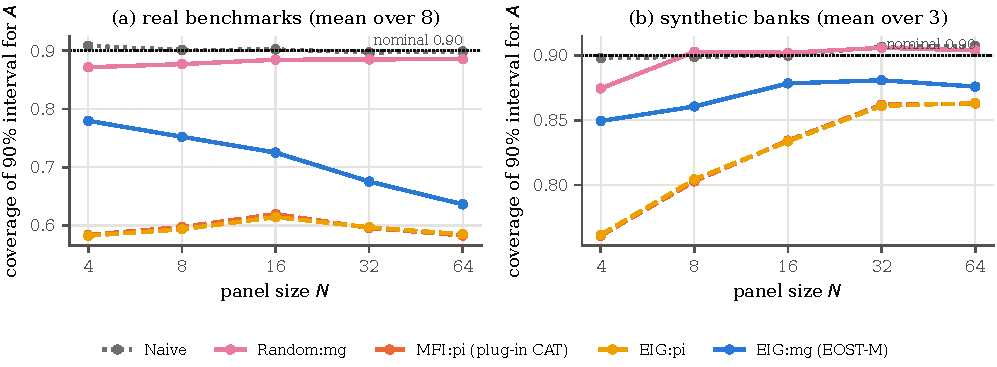
\includegraphics[width=\linewidth]{figures/coverage.pdf}
\caption{Coverage of the 90\% interval for the full-bank score, averaged over steps, targets and benchmarks, as a function of the panel size. Dotted line: nominal level.}
\label{fig:coverage}
\end{figure}

\subsection{Synthetic banks}\label{sec:synthetic}
\ResultsSynthetic

\begin{figure}[tbp]
\centering
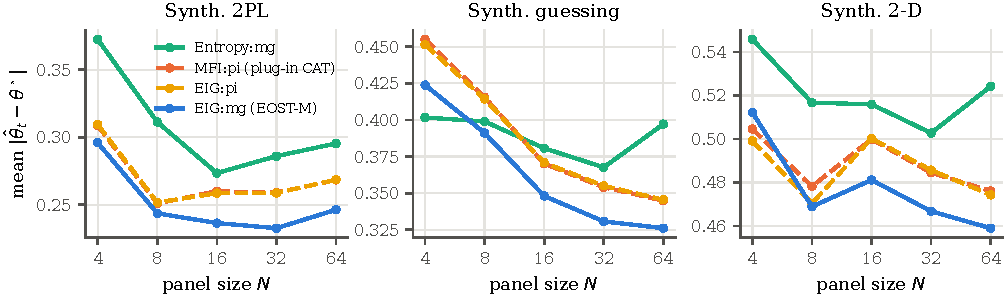
\includegraphics[width=\linewidth]{figures/synthetic_theta.pdf}
\caption{Error of the ability estimate with respect to the true generating ability on the three synthetic banks (well-specified 2PL; 60\% of items with a 0.25 guessing floor; two correlated ability dimensions), averaged over the 100-item test.}
\label{fig:synth}
\end{figure}

\subsection{Sensitivity analyses}\label{sec:sensitivity}
\ResultsSensitivity

\begin{table}[tbp]
\centering\footnotesize
\caption{Sensitivity analyses (30 targets, 3 replicates; main analysis for reference). Median relative improvement of EIG:mg across confirmatory benchmarks, in \%, [benchmarks improved / tested], and mean coverage of EOST-M's 90\% score interval. $^{\dagger}$Specified in the frozen plan, but its joint MAP is degenerate (the common discrimination diverges; Section~\ref{sec:sensitivity}), so its contrasts are not interpreted. $^{\ddagger}$Post hoc: common discrimination with prior $\log a\sim\mathcal N(0,0.05^2)$.}
\label{tab:sens}
\setlength{\tabcolsep}{3.5pt}
\begin{tabular}{@{}lrlllll@{}}
\toprule
Variant & $N$ & H1 log loss & H2 log loss & H3 IAE & H4 cov.\ gap & cov. \\
\midrule
main (EB prior, 2PL) & 8 & $+1.9$ [8/8] & $+5.2$ [8/8] & $+54.4$ [8/8] & $+44.2$ [8/8] & 0.75 \\
main (EB prior, 2PL) & 64 & $+1.8$ [6/6] & $+1.1$ [6/6] & $+62.1$ [6/6] & $+10.3$ [6/6] & 0.64 \\
fixed item prior & 8 & $+2.3$ [8/8] & $+2.8$ [5/8] & $+46.4$ [8/8] & $+35.8$ [5/8] & 0.70 \\
fixed item prior & 64 & $+2.2$ [6/6] & $+0.7$ [4/6] & $+63.2$ [6/6] & $+9.1$ [5/6] & 0.63 \\
near-duplicates removed & 8 & $+2.0$ [5/5] & $+6.1$ [5/5] & $+49.1$ [5/5] & $+46.2$ [4/5] & 0.73 \\
near-duplicates removed & 64 & $+2.2$ [5/5] & $+1.0$ [5/5] & $+66.4$ [5/5] & $+6.9$ [3/5] & 0.64 \\
\midrule
one-parameter$^{\dagger}$ & 8 & $-0.5$ [4/8] & $+38.9$ [8/8] & $-95.6$ [1/8] & $-3.8$ [3/8] & 0.15 \\
one-parameter$^{\dagger}$ & 64 & $-0.4$ [3/6] & $+45.0$ [4/6] & $-140.1$ [1/6] & $+0.9$ [4/6] & 0.20 \\
\midrule
one-parameter, regularized$^{\ddagger}$ & 8 & $+0.4$ [7/8] & $+0.7$ [7/8] & $+51.8$ [8/8] & $+14.3$ [8/8] & 0.84 \\
one-parameter, regularized$^{\ddagger}$ & 64 & $-0.2$ [2/6] & $0.0$ [3/6] & $+44.8$ [6/6] & $-3.3$ [3/6] & 0.81 \\
\bottomrule
\end{tabular}
\end{table}


\subsection{Post hoc probes that motivated study 2}\label{sec:strong}
After all frozen runs, three post hoc analyses with decision rules recorded before running
probed the main result: strong baselines, a regularization path of the discrimination prior
and a decomposition of interval coverage. \ResultsStrong

Because the regularized Rasch-type test is a strong competitor found after the fact,
study~2 tests it, together with a Bayesian CAT that also integrates the calibrators'
abilities, under a new frozen plan.

\IfFileExists{tables/posthoc.tex}{\begin{table}[tbp]
\centering\footnotesize
\caption{Post hoc comparison with strong baselines (not in the frozen plan; same targets, replicates, holdouts and calibration panels as the confirmatory study; decision rules recorded before the runs). Median relative improvement of EOST-M (EIG:mg) over each baseline across the eight benchmarks, in \%, with [benchmarks with a Holm-significant difference favouring EOST-M / favouring the baseline], Holm over this post hoc family, so that the counts for MFI:pi differ from Table~\ref{tab:confirm}; last column: mean coverage of the baseline's 90\% score interval at $N=8$.}
\label{tab:posthoc}
\setlength{\tabcolsep}{2.3pt}
\begin{tabular}{@{}lcccccc@{}}
\toprule
 & \multicolumn{3}{c}{holdout log loss} & score IAE & $|\mathrm{cov}-0.9|$ & cov. \\
\cmidrule(lr){2-4}\cmidrule(lr){5-5}\cmidrule(lr){6-6}\cmidrule(lr){7-7}
Policy & $N=4$ & $N=8$ & $N=16$ & $N=8$ & $N=8$ & $N=8$ \\
\midrule
EOST-M (EIG:mg), reference & -- & -- & -- & -- & -- & 0.75 \\
\midrule
plug-in 2PL (MFI:pi) & $+7.1$ [8/0] & $+5.2$ [5/0] & $+3.6$ [2/0] & $+7.5$ [1/0] & $+44.2$ [5/0] & 0.60 \\
plug-in posterior-mean 2PL, MFI & $+20.4$ [8/0] & $+15.5$ [7/0] & $+10.0$ [7/0] & $+7.3$ [2/0] & $+52.5$ [6/0] & 0.54 \\
plug-in posterior-mean 2PL, EIG & $+21.2$ [8/0] & $+14.7$ [7/0] & $+9.8$ [7/0] & $+7.7$ [2/0] & $+53.7$ [6/0] & 0.53 \\
plug-in regularized 1PL, MFI & $+2.9$ [4/0] & $+2.1$ [4/0] & $+3.3$ [5/0] & $+2.9$ [2/0] & $-25.9$ [0/0] & 0.81 \\
marginal regularized 1PL, EIG & $+1.0$ [3/0] & $+1.8$ [5/0] & $+2.8$ [4/0] & $+6.7$ [2/0] & $-54.0$ [0/1] & 0.83 \\
expected Fisher information (EFI:mg) & $0.0$ [0/0] & $0.0$ [0/0] & $0.0$ [0/0] & $+0.9$ [0/0] & $-3.0$ [0/0] & 0.76 \\
\bottomrule
\end{tabular}
\end{table}
}{}

\IfFileExists{figures/shrinkage_path.pdf}{%
\begin{figure}[tbp]
\centering
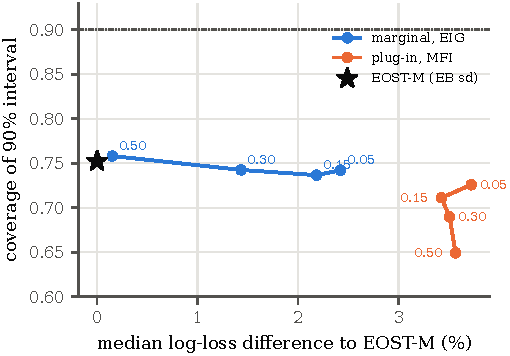
\includegraphics[width=0.55\linewidth]{figures/shrinkage_path.pdf}
\caption{Exploratory regularization path ($N=8$; planned before running): EOST-M's calibration with the prior standard deviation of $\log a$ fixed to the value next to each point instead of its empirical-Bayes estimate, for the marginal model with EIG and the plug-in model with MFI. Horizontal axis: median over benchmarks of the relative held-out log-loss difference to EOST-M; vertical axis: mean coverage of the 90\% score interval (dotted: nominal).}
\label{fig:shrink}
\end{figure}}{}

\IfFileExists{tables/coverage_decomp.tex}{\begin{table}[tbp]
\centering\footnotesize
\caption{Where the coverage of the 90\% score interval comes from (exploratory analysis of the post hoc runs, planned before computing; $N=8$). Coverage and score IAE (in percentage points) of EOST-M (EIG:mg) and of the regularized Rasch-type plug-in test (MFI:1pr), median over targets of the ratio of their mean interval widths (Rasch-type over EOST-M; Holm-significant on 8 of 8 benchmarks), and ratio of mean interval width to score IAE for plug-in 2PL (MFI:pi), EOST-M, the Rasch-type test and the marginal regularized one-parameter model (EIG:1prmg, column 1PL:mg). A calibrated 90\% interval for unbiased Gaussian errors has ratio $2\cdot1.645/\sqrt{2/\pi}=4.12$.}
\label{tab:covdecomp}
\setlength{\tabcolsep}{3pt}
\begin{tabular}{@{}lccccccccc@{}}
\toprule
 & \multicolumn{2}{c}{coverage} & width & \multicolumn{2}{c}{score IAE} & \multicolumn{4}{c}{width / IAE} \\
\cmidrule(lr){2-3}\cmidrule(lr){4-4}\cmidrule(lr){5-6}\cmidrule(l){7-10}
Benchmark & EOST-M & Rasch & ratio & EOST-M & Rasch & MFI:pi & EOST-M & Rasch & 1PL:mg \\
\midrule
GSM8K & 0.70 & 0.78 & 1.12 & 4.4 & 4.1 & 2.62 & 2.89 & 3.34 & 3.33 \\
ARC-C & 0.74 & 0.87 & 1.44 & 2.9 & 3.0 & 2.20 & 2.97 & 3.97 & 3.83 \\
HellaSwag & 0.76 & 0.79 & 1.14 & 1.8 & 1.7 & 2.00 & 2.88 & 3.21 & 3.46 \\
WinoGrande & 0.75 & 0.75 & 1.52 & 2.9 & 4.2 & 1.84 & 2.97 & 3.06 & 2.99 \\
MMLU & 0.77 & 0.81 & 1.76 & 3.2 & 5.3 & 1.90 & 3.22 & 3.40 & 3.68 \\
SWE-bench V. & 0.76 & 0.81 & 1.20 & 3.5 & 3.5 & 2.39 & 2.98 & 3.51 & 3.70 \\
LiveCodeBench & 0.76 & 0.81 & 1.08 & 2.9 & 2.7 & 2.26 & 3.11 & 3.53 & 3.83 \\
CRUXEval-O & 0.77 & 0.86 & 1.39 & 3.1 & 3.4 & 2.29 & 3.17 & 3.85 & 3.89 \\
\bottomrule
\end{tabular}
\end{table}
}{}
